\chapter{Diseño e implementación de un orquestador para tareas de tiempo real}

En los capítulos anteriores, se ha presentado el concepto de la Industria 4.0 y
los problemas que plantea, indicando que el paradigma del \textit{fog computing}
y las tecnologías de virtualización pueden ser una solución factible para
conseguir su implantación. Para apoyar este planteamiento, se ha decidido
implementar una herramienta de orquestación de tareas de tiempo real sobre
entornos distribuidos que sirva como prueba de concepto. En este capítulo, se
detalla el proceso seguido para su desarrollo, justificando las decisiones
de diseño tomadas y mostrando los de detalles más relevantes de la
implementación. Para terminar, se muestra una caracterización inicial del
rendimiento de la herramienta desarrollada.

\section{Objetivos y requisitos}

Como ya se ha explicado, la llegada de la Industria 4.0 supone un aumento muy
grande en la cantidad de datos generados en las plantas debido al IoT
industrial, datos que son necesarios para poder obtener gemelos digitales con un
nivel de detalle suficiente. Los nuevos sistemas ciber-físicos necesitan, por
tanto, procesar todos estos datos en tiempo real para poder tomar decisiones de
control en base a los mismos y garantizar una operación eficiente. Para ello, es
necesario poseer una capacidad de procesamiento elevada, mayor de la que
cualquier dispositivo individual pueda aportar. Aunque la computación en la nube
pueda parecer una solución natural a este problema, la enorme carga que pondría
sobre la red la constante transmisión de cantidades de datos tan grandes, así
como la latencia resultante de estas comunicaciones, hacen que no podamos
considerar esta plataforma como apropiada para dar cobijo a tareas con
restricciones temporales. En la sección \ref{sec:cloud-fog-edge}, se introduce
el paradigma \textit{fog} como una extensión de la nube más cercana a las
fuentes de datos. Según este modelo, los datos generados por los dispositivos
del borde de la red son procesados en nodos ubicados en la misma red local.
Aunque la potencia combinada de los dispositivos que conformen esta capa
\textit{fog} será menor que la que encontramos en la nube, puede ser suficiente
para las tareas de análisis de datos y toma de decisiones que se deben realizar
en las plantas, reduciendo así la presión sobre la red y garantizando unos
tiempos de respuesta muy inferiores.

Debido a esto, el modelo \textit{fog} se plantea como una posible plataforma
para la implementación de los nuevos sistemas ciber-físicos. Las tareas de
control industrial deben, entonces, distribuirse por los nodos de la capa
\textit{fog} de forma dinámica para dar respuesta a la carga de trabajo en todo
momento. Para que esta distribución de procesos sobre los nodos se produzca de
manera eficiente, es necesario hacer uso de las tecnologías de virtualización,
las cuales ya sirven para solucionar una problemática similar en la nube. Al
virtualizar los procesos, se abstraen las capas inferiores como son el hardware
o el sistema operativo, facilitando el despliegue de los mismos sobre
dispositivos con características dispares y unificando su desarrollo, dado que
no es necesario implementarlos para cada plataforma distinta). Así, se facilita
la escalabilidad de los procesos para dar respuesta a los cambios en la demanda.
En la sección \ref{sec:virtualization}, planteamos el uso de contenedores en vez
de máquinas virtuales para esto, apoyándonos en su carácter más liviano y su
mejor rendimiento para operaciones de entrada y salida.

Por tanto, en el modelo planteado es necesario desplegar las tareas de control
en forma de contenedores. Para explorar más este concepto, hemos decidido
implementar una herramienta que permita realizar esto sobre múltiples nodos. Los
objetivos de esta herramienta son:

\begin{table}[H]
    \centering
    \begin{tabular}{ |>{\columncolor[gray]{0.8}}l|p{0.7\textwidth}| }
        \hline
        Nombre      & Gestión de nodos                                       \\
        \hline
        Importancia & Alta                                                   \\
        \hline
        Descripción & Llevar un control de los dispositivos que conforman la
        capa \textit{fog} es una parte esencial de la implantación de este
        modelo.                                                              \\
        \hline
    \end{tabular}
    \caption{Objetivo 01 - Gestión de nodos}
    \label{tab:04-obj01}
\end{table}

\begin{table}[H]
    \centering
    \begin{tabular}{ |>{\columncolor[gray]{0.8}}l|p{0.7\textwidth}| }
        \hline
        Nombre      & Gestión de tareas                                          \\
        \hline
        Importancia & Alta                                                       \\
        \hline
        Descripción & Las distintas tareas que se deben ejecutar sobre los nodos
        de la capa \textit{fog} deben estar recopiladas y centralizadas en el
        sistema.                                                                 \\
        \hline
    \end{tabular}
    \caption{Objetivo 02 - Gestión de tareas}
    \label{tab:04-obj02}
\end{table}

\begin{table}[H]
    \centering
    \begin{tabular}{ |>{\columncolor[gray]{0.8}}l|p{0.7\textwidth}| }
        \hline
        Nombre      & Orquestación de tareas                                \\
        \hline
        Importancia & Muy alta                                              \\
        \hline
        Descripción & El sistema debe permitir a los usuarios desplegar las
        tareas definidas sobre los nodos de manera sencilla, controlando siempre
        que la ejecución de las tareas sobre cada nodo concreto sea viable. \\
        \hline
    \end{tabular}
    \caption{Objetivo 03 - Orquestación de tareas}
    \label{tab:04-obj03}
\end{table}

\begin{table}[H]
    \centering
    \begin{tabular}{ |>{\columncolor[gray]{0.8}}l|p{0.7\textwidth}| }
        \hline
        Nombre      & Uso de software libre                                      \\
        \hline
        Importancia & Media                                                      \\
        \hline
        Descripción & Como parte de nuestro compromiso con el software libre, el
        sistema desarrollador deberá hacer uso siempre que sea posible de
        tecnologías abiertas.                                                    \\
        \hline
    \end{tabular}
    \caption{Objetivo 04 - Uso de software libre}
    \label{tab:04-obj04}
\end{table}

A partir de estos objetivos, se han concretado una serie de requisitos que
deberá satisfacer la herramienta desarrollada.

\begin{table}[H]
    \centering
    \begin{tabular}{ |>{\columncolor[gray]{0.8}}l|p{0.5\textwidth}| }
        \hline
        Nombre                 & Añadir un nuevo nodo                       \\
        \hline
        Objetivos relacionados & \ref{tab:04-obj01}                         \\
        \hline
        Descripción            & Un usuario debe poder añadir al sistema un
        nuevo nodo que represente a un dispositivo de la capa \textit{fog}. Los
        datos proporcionados para el nuevo nodo deben permitir la conexión al
        mismo por SSH.                                                      \\
        \hline
    \end{tabular}
    \caption{Requisito 01 - Añadir un nuevo nodo}
    \label{tab:04-req01}
\end{table}

\begin{table}[H]
    \centering
    \begin{tabular}{ |>{\columncolor[gray]{0.8}}l|p{0.5\textwidth}| }
        \hline
        Nombre                 & Obtener datos de los nodos                      \\
        \hline
        Objetivos relacionados & \ref{tab:04-obj01}                              \\
        \hline
        Descripción            & Un usuario debe poder obtener información sobre
        los nodos que hay registrados en el sistema, tanto de forma colectiva como
        detallada para un nodo concreto.                                         \\
        \hline
    \end{tabular}
    \caption{Requisito 02 - Obtener datos de los nodos}
    \label{tab:04-req02}
\end{table}

\begin{table}[H]
    \centering
    \begin{tabular}{ |>{\columncolor[gray]{0.8}}l|p{0.5\textwidth}| }
        \hline
        Nombre                 & Modificar un nodo                               \\
        \hline
        Objetivos relacionados & \ref{tab:04-obj01}                              \\
        \hline
        Descripción            & Un usuario debe poder actualizar la información
        relativa a un nodo ya registrado en el sistema si fuera necesario.       \\
        \hline
    \end{tabular}
    \caption{Requisito 03 - Modificar un nodo}
    \label{tab:04-req03}
\end{table}

\begin{table}[H]
    \centering
    \begin{tabular}{ |>{\columncolor[gray]{0.8}}l|p{0.5\textwidth}| }
        \hline
        Nombre                 & Eliminar un nodo                              \\
        \hline
        Objetivos relacionados & \ref{tab:04-obj01}                            \\
        \hline
        Descripción            & Un usuario debe poder eliminar del sistema un
        nodo cuando sea necesario.                                             \\
        \hline
    \end{tabular}
    \caption{Requisito 04 - Eliminar un nodo}
    \label{tab:04-req04}
\end{table}

\begin{table}[H]
    \centering
    \begin{tabular}{ |>{\columncolor[gray]{0.8}}l|p{0.5\textwidth}| }
        \hline
        Nombre                 & Añadir una nueva tarea                         \\
        \hline
        Objetivos relacionados & \ref{tab:04-obj02}                             \\
        \hline
        Descripción            & Un usuario debe poder añadir al sistema tareas
        de tiempo real para su posterior despliegue sobre los nodos del mismo.
        Se deben aportar, por tanto, tanto los ficheros con la tarea como los
        atributos relativos a sus restricciones temporales.                     \\
        \hline
    \end{tabular}
    \caption{Requisito 05 - Añadir una nueva tarea}
    \label{tab:04-req05}
\end{table}

\begin{table}[H]
    \centering
    \begin{tabular}{ |>{\columncolor[gray]{0.8}}l|p{0.5\textwidth}| }
        \hline
        Nombre                 & Obtener datos de las tareas              \\
        \hline
        Objetivos relacionados & \ref{tab:04-obj02}                       \\
        \hline
        Descripción            & Un usuario debe poder ver la información
        relativa a las tareas registradas en el sistema.                  \\
        \hline
    \end{tabular}
    \caption{Requisito 06 - Obtener datos de las tareas}
    \label{tab:04-req06}
\end{table}


\begin{table}[H]
    \centering
    \begin{tabular}{ |>{\columncolor[gray]{0.8}}l|p{0.5\textwidth}| }
        \hline
        Nombre                 & Modificar una tarea                           \\
        \hline
        Objetivos relacionados & \ref{tab:04-obj02}                            \\
        \hline
        Descripción            & Un usuario debe poder actualizar una tarea ya
        presente en el sistema si fuera necesario.                             \\
        \hline
    \end{tabular}
    \caption{Requisito 07 - Modificar una tarea}
    \label{tab:04-req07}
\end{table}

\begin{table}[H]
    \centering
    \begin{tabular}{ |>{\columncolor[gray]{0.8}}l|p{0.5\textwidth}| }
        \hline
        Nombre                 & Eliminar una tarea                           \\
        \hline
        Objetivos relacionados & \ref{tab:04-obj02}                           \\
        \hline
        Descripción            & Un usuario debe poder eliminar una tarea del
        sistema.                                                              \\
        \hline
    \end{tabular}
    \caption{Requisito 08 - Eliminar una tarea}
    \label{tab:04-req08}
\end{table}

\begin{table}[H]
    \centering
    \begin{tabular}{ |>{\columncolor[gray]{0.8}}l|p{0.5\textwidth}| }
        \hline
        Nombre                 & Desplegar una tarea en un nodo            \\
        \hline
        Objetivos relacionados & \ref{tab:04-obj03}                        \\
        \hline
        Descripción            & Un usuario debe poder desplegar una tarea
        registrada en el sistema sobre un nodo también registrado.         \\
        \hline
    \end{tabular}
    \caption{Requisito 09 - Desplegar una tarea en un nodo}
    \label{tab:04-req09}
\end{table}

\begin{table}[H]
    \centering
    \begin{tabular}{ |>{\columncolor[gray]{0.8}}l|p{0.5\textwidth}| }
        \hline
        Nombre                 & Eliminar una tarea de un nodo            \\
        \hline
        Objetivos relacionados & \ref{tab:04-obj03}                       \\
        \hline
        Descripción            & Un usuario debe poder eliminar una tarea
        previamente desplegada en un nodo cuando sea necesario.           \\
        \hline
    \end{tabular}
    \caption{Requisito 10 - Eliminar una tarea de un nodo}
    \label{tab:04-req10}
\end{table}

\begin{table}[H]
    \centering
    \begin{tabular}{ |>{\columncolor[gray]{0.8}}l|p{0.5\textwidth}| }
        \hline
        Nombre                 & Garantizar la viabilidad de los conjuntos de tareas \\
        \hline
        Objetivos relacionados & \ref{tab:04-obj03}                                  \\
        \hline
        Descripción            & El sistema debe de garantizar en todo momento y
        en la medida de lo posible que las tareas que se ejecutan sobre un nodo
        dado son viables.                                                            \\
        \hline
    \end{tabular}
    \caption{Requisito 11 - Garantizar la viabilidad de los conjuntos de tareas}
    \label{tab:04-req11}
\end{table}

\begin{table}[H]
    \centering
    \begin{tabular}{ |>{\columncolor[gray]{0.8}}l|p{0.5\textwidth}| }
        \hline
        Nombre                 & Despliegue usando contenedores                 \\
        \hline
        Objetivos relacionados & \ref{tab:04-obj03}                             \\
        \hline
        Descripción            & El despliegue de las tareas sobre los nodos se
        debe realizar mediante contenedores.                                    \\
        \hline
    \end{tabular}
    \caption{Requisito 12 - Despliegue usando contenedores}
    \label{tab:04-req12}
\end{table}

\section{Diseño del sistema}

A la hora de abordar el diseño de la herramienta, se nos planteaban varias
posibilidades. La solución más sencilla podría consistir de una aplicación
monolítica, de escritorio o web, que aglutinase toda la funcionalidad recogida
en los requisitos detallados en la sección anterior. Una aplicación monolítica
de este tipo, aunque no siempre es una mala opción, plantea varios problemas
como son su difícil escalabilidad o la complejidad creciente conforme se añaden
funcionalidades, lo que incrementa los costes de desarrollo y mantenimiento.
Además, el sistema que se desea crear se visualiza siendo usado por varios
usuarios. Se podría pensar, por ejemplo, en ingenieros de una fábrica que se
encargan del desarrollo y mantenimiento de sus sistemas de control, cada uno
usando su propio PC para llevar a cabo estas tareas a través de nuestra
herramienta. En una situación como esa, usar una aplicación monolítica es
inviable, dado que los usuarios deben trabajar de forma concurrente sobre un
conjunto de datos común.

La manera más sencilla para permitir esta colaboración y conseguir que todos los
usuarios trabajen sobre una misma base consiste en aplicar un modelo de
cliente-servidor. El sistema se modulariza, encapsulando la funcionalidad más
importante en un servidor y relegando las aplicaciones que usan los usuarios a
simples cascarones encargados de proporcionar una interfaz entre las
funcionalidades del sistema y ellos mismos. Una arquitectura de este tipo hace
más fácil controlar el acceso concurrente a los datos, evitando problemas de
integridad e incoherencia en los mismos. Además, debido a que los clientes no
tienen tantas responsabilidades, acaban siendo más simples y livianos, lo que
facilita su instalación en las máquinas de los usuarios. Es por todas estas
razones que se ha escogido la arquitectura cliente-servidor para el diseño del
sistema. En la figura \ref{fig:04-architecture} se puede ver un diagrama del
diseño propuesto para el sistema. Aquí se puede ver como el servidor contiene
toda la lógica relativa a los nodos, las tareas y el despliegue de éstas. Aunque
se podría haber planteado la separación de esta lógica en varios microservicios,
esta opción se descartó debido a que no se espera que el sistema tenga que ser
usado por muchos usuarios a la vez ni su carga pueda elevarse de forma
considerable, por lo que los beneficios de escalabilidad que este tipo de diseño
podría aportar son innecesarios y se ven enormemente contrarrestados por la
complejidad que añaden.

\begin{figure}
    \centering
    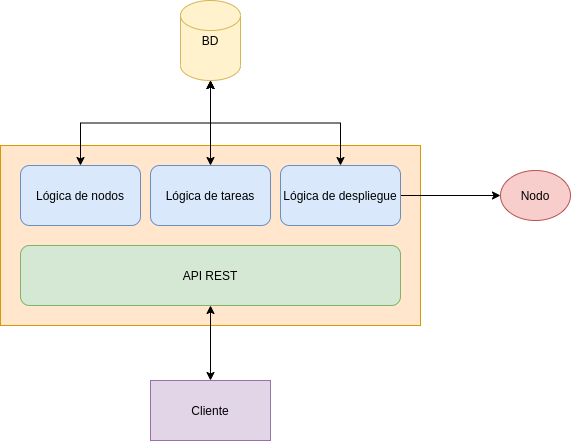
\includegraphics[width=0.8\textwidth]{04-implementation/architecture.png}
    \caption{Diagrama de arquitectura del sistema}
    \label{fig:04-architecture}
\end{figure}

Volviendo a la figura \ref{fig:04-architecture}, apreciamos que el servidor
también controla el acceso a la base de datos donde se almacena toda la
información sobre los nodos y las tareas. Para esta base de datos, como ya se
indicó en la sección \ref{sec:tools}, se ha decidido MongoDB, que es un gestor
de bases de datos documentales y no estructuradas. También se puede comprobar en
el diagrama que el servidor expone todas las funcionalidades del sistema a
través de una API (\textit{Application Programming Interface}). Esta API sigue
el patrón arquitectónico REST (\textit{REpresentation State Transfer}), el cuál
fue introducido en el año 2000 por Roy Fielding en su tesis doctoral
\cite{fielding_architectural_2000}. Simplificando los conceptos que se
desarrollan en esta tesis, podemos identificar las siguientes características
fundamentales del patrón REST:

\begin{itemize}
    \item La interfaz se diseña en torno a recursos, los cuáles son conjuntos de
          información.
    \item Cada recurso está identificado de forma única mediante una URI.
    \item Las operaciones se realizan mediante peticiones HTTP hacia la URI del
          recurso objetivo.
    \item La operación a realizar viene definida por el verbo HTTP usado en la
          petición (\texttt{GET}, \texttt{POST}, \texttt{PUT}, \texttt{PATCH} o
          \texttt{DELETE}).
    \item El servidor no almacena estado alguno, de forma que cada petición debe
          contener toda la información necesaria como para poder darle respuesta.
    \item Para la transferencia de información, se utilizan formatos bien
          definidos como JSON o XML.
\end{itemize}

La aplicación del patrón REST al diseño de interfaces hace que sea más sencillo
estructurar el acceso a la información que contiene un servicio concreto, además
de simplificar también el flujo de trabajo entre cliente y servidor. Para
aplicar REST al diseño de un servicio concreto, se debe identificar cuáles son
los recursos con los que trabaja y qué operaciones permite sobre los mismos. En
el caso de nuestro sistema, tenemos los recursos detallados en las tablas
\ref{tab:04-node_resource} y \ref{tab:04-task_resource}.

\begin{table}[H]
    \centering
    \begin{tabular}{ |>{\columncolor[gray]{0.8}}l|p{0.8\textwidth}| }
        \hline
        Recurso   & Nodo           \\
        \hline
        Atributos &
        \begin{itemize}
            \item ID
            \item Nombre
            \item Dirección IP
            \item Usuario (utilizado para la conexión SSH)
            \item CPU (modelo del procesador)
            \item Arquitectura de CPU (p. ej., \texttt{ARMv7})
            \item Número de núcleos de la CPU
            \item Frecuencia de reloj
            \item RAM
            \item Dispositivos (p. ej., \texttt{/dev/null})
            \item Tareas (que se están ejecutando en el nodo)
        \end{itemize} \\
        \hline
    \end{tabular}
    \caption{Definición del recurso nodo}
    \label{tab:04-node_resource}
\end{table}

\begin{table}[H]
    \centering
    \begin{tabular}{ |>{\columncolor[gray]{0.8}}l|p{0.8\textwidth}| }
        \hline
        Recurso   & Tarea          \\
        \hline
        Atributos &
        \begin{itemize}
            \item ID
            \item Nombre
            \item Tiempo de ejecución (\textit{runtime})
            \item Límite de tiempo (\textit{deadline})
            \item Período (\textit{period})
            \item Dispositivos (a los que necesita acceder)
            \item Capacidades (p. ej., \texttt{SYS\_NICE})
            \item ID del desplegable (fichero tar con código fuente y \texttt{Dockerfile})
        \end{itemize} \\
        \hline
    \end{tabular}
    \caption{Definición del recurso tarea}
    \label{tab:04-task_resource}
\end{table}

Como ya se ha indicado, aplicar una arquitectura cliente-servidor como esta
permite reducir al máximo la lógica que contienen los clientes, los cuáles solo
tienen que ocuparse de mostrar la interfaz, comprobar las entradas de los
usuarios y realizar la comunicación con el servidor. Además, el hecho de que el
servidor exponga una API estandarizada facilita enormemente la implementación de
múltiples tipos de aplicaciones cliente, incluso para distintas plataformas (p.
ej., móvil, web o escritorio). Estos clientes sencillamente tienen que consumir
recursos de la interfaz y pueden ofrecer a sus usuarios exactamente las mismas
funcionalidades que los demás. Esta separación de responsabilidades facilita
también el desarrollo y mantenimiento del software, ya que se trata de partes
completamente independientes y separadas que solo deben atenerse a la
especificación de la interfaz mediante la que se conectan.

Por último, también se ha decidido en esta fase de diseño implementar una imagen
Docker, que es el motor de contenedores usado por el sistema, para facilitar el
despliegue de tareas de tiempo real usando el sistema planteado. El
funcionamiento de esta imagen, así como los detalles de diseño e implementación
de las demás partes del sistema, se explican de forma extensiva en las
siguientes secciones de este capítulo.

\section{Servidor maestro}

\subsection{Diseño}

\subsection{Implementación}

\subsection{Prueba}

\subsection{Integración contínua}

\section{Cliente de terminal}

\subsection{Diseño}

\subsection{Implementación}

\subsection{Prueba}

\subsection{Integración contínua}

\section{Imagen base}

\subsection{Diseño}

\subsection{Implementación}

\subsection{Prueba}

\subsection{Integración contínua}

\section{Análisis del rendimiento}